\documentclass{standalone}

\usepackage{tikz}
    \usetikzlibrary{arrows.meta}

\usepackage{graphicx} % Работа с графикой \includegraphics{}
\graphicspath{{./images/img1/}} % картинки в папке ./images/img1/
    
\begin{document}

\begin{tikzpicture}
    %\draw[help lines, green] (-3,-3) grid (9,3);
    %\draw[help lines, step=0.1] (-3,-3) grid (9,3);
    \node at(-2.5,-2.5){1};
    \node at(2.5,-2.5){2};
    \node at(2.5,2.3){3};
    \node at(-2.5,2.3){4}; %Вершины P
    \node at(-1.5,-1.6){$P_1$};
    \node at(1.5,-1.5){$P_2$};
    \node at(1.3,1.5){$P_3$};
    \node at(-1.6,1.3){$P_4$};
    \node at(-0.3,0){$P_5$}; %Копии P_i
    \node at(-2,-2.2){\footnotesize{1}};
    \node at(-1,-2.2){\footnotesize{2}};
    \node at(-1,-1.2){\footnotesize{3}};
    \node at(-2,-1.3){\footnotesize{4}}; %Вершины P_1
    \node at(2,-2.1){\footnotesize{4}};
    \node at(2.3,-0.9){\footnotesize{1}};
    \node at(0.9,-0.8){\footnotesize{2}};
    \node at(0.7,-2){\footnotesize{3}}; %Вершины P_2
    \node at(2,1.8){\footnotesize{2}};
    \node at(0.8,2.2){\footnotesize{3}};
    \node at(0.5,1.1){\footnotesize{4}};
    \node at(1.7,0.7){\footnotesize{1}}; %Вершины P_3
    \node at(-2.2,0.9){\footnotesize{2}};
    \node at(-2.1,1.7){\footnotesize{1}};
    \node at(-1.3,0.8){\footnotesize{3}};
    \node at(-1.2,1.6){\footnotesize{4}}; %Вершины P_4
    \node at(-0.7,-0.7){\footnotesize{1}};
    \node at(0.4,-0.4){\footnotesize{2}};
    \node at(0.2,0.6){\footnotesize{3}};
    \node at(-1,0.4){\footnotesize{4}}; %Вершины P_5
    \node  at (0,0) 
        {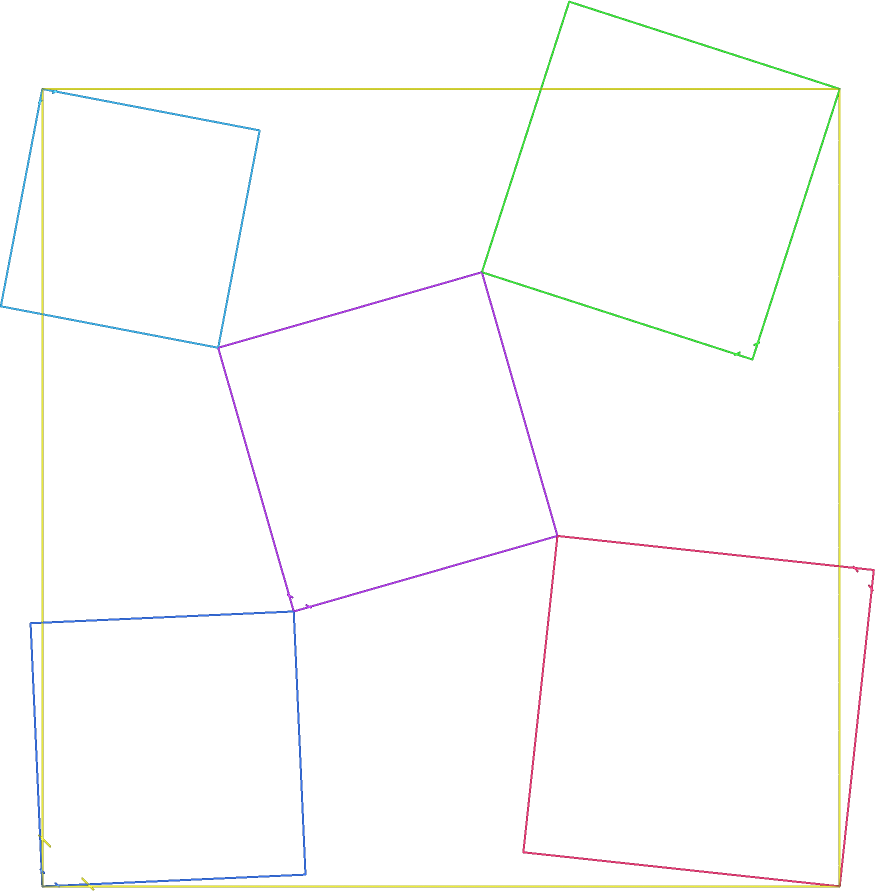
\includegraphics[width=4.8cm]{p1s.png}};
    \node[shape=circle, draw, red, line width=1pt] (a1) at ( 5,-2) {1};
    \node[shape=circle, draw, line width=1pt] (a2) at (8.5,-2) {2};
    \node[shape=circle, draw, line width=1pt] (a3) at (8.5,1.5) {3};
    \node[shape=circle, draw, line width=1pt] (a4) at (5,1.5) {4};
    \path[->,>={Latex[length=8pt]},line width=1pt] 
        (a3) edge node[left]{3} (a2)
        (a2) edge node[above right]{2} (a4)
        (a4) edge node[left]{4} (a1)
        (a1) edge[red, thick, loop left, distance=1.5cm] node[shift={(0.7,0.4)}]{1} (a1);
\end{tikzpicture}

\end{document}